\label{NN}
A neural  network is a type of machine learning model, which is represented
through a hierarchical structure of layers. Each layer consists of a fixed set
of units or neurons with adaptable parameters, which can be changed during
training. When some input data is passed into the network, each successive layer
uses the output from the previous layer as input. The process is then repeated
until an output layer has been reached. The interpretation of the output from a
network depends on the modeling problem. A common one is the \emph{multiclass}
problem, where there are $N$ prediction classes. The goal of the neural network
is then to predict which class the input data belongs to. In such a case the
output is interpreted as probabilities.\newline \newline 
How each layer process the input depends on the type of layer, where this thesis
will show the process for a fully-connected- and convolutional layer. Before
doing so, introducing some terminology is needed. When a neural network consists
solely of fully-connected layers, it is called a \emph{multilayer perceptron}
and if a neural network has at least one convolutional layer, but maybe one or
more fully-connected, it is called a \emph{convolutional network}. The
architecture of a convolutional network usually consists of convolutional layers
at the beginning of the network and ends with a number of fully-connected layers
at the end. The next section will show how information is processed in a
multilayer perceptron and a derivation showing the backpropagation algorithm
applied to a multilayer perceptron of an arbitrary depth, which in the
subsequent section will be extended to a convolutional network. 

\newpage 
\section{Multilayer perceptron}
\label{sec:mlp}
Multilayer perceptrons (MLP) are the simplest form of neural networks, where
every output from a given layer is connected to every single neuron of the next
layer. Figure \ref{fig:mlp2} shows a MLP with two layers\footnote{There is some
	confusion about counting layers in a network, where some would call this network
	a three layer network. Using same terminology as C. Bishop I will also call this
	a two-layer network, since there are two layers with weights.}. 
\begin{figure}[!htbp]
	\centering 
	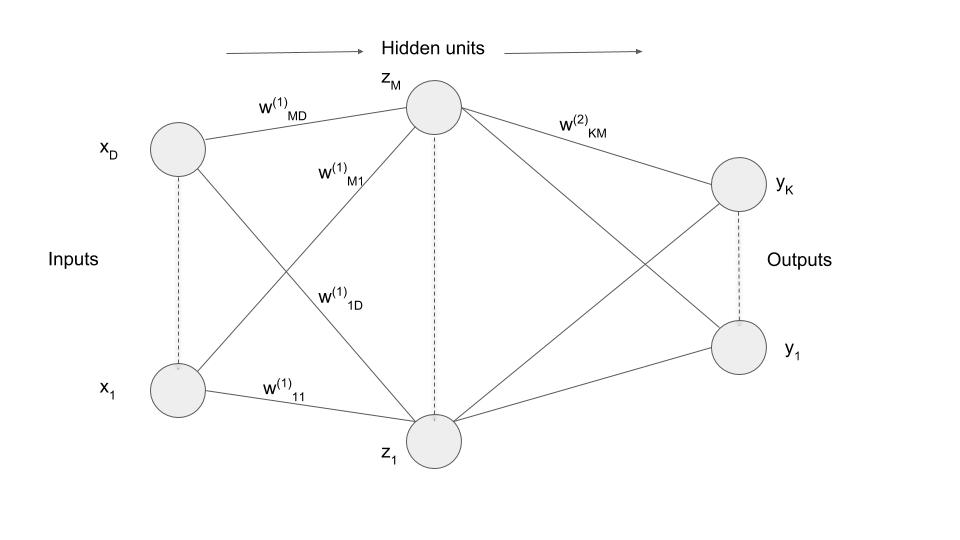
\includegraphics[width=\textwidth]{pics/nn}
	\caption{A 2-layer MLP network showing only the outer most neurons.
		(source:\cite[ch. 5]{Bishop:2006:PRM:1162264})}
	\label{fig:mlp2}
\end{figure}\newline 
Using Figure \ref{fig:mlp2} as an example we can express the first layer with
$M$ neurons as having $M$ linear combinations with $D$ inputs. Using this
formulation and letting $x_1, x_2,  \cdots, x_D$ be the input into the network
in Figure \ref{fig:mlp2}, we can write the first layer calculation as:
\begin{equation}
\label{eq:layer1}
a_j = \sum_{i=1}^{D} w_{ji}^{(1)}x_i + b^{(1)}_{j} 
\end{equation}
where $j \in \{1...M\}$, that is each neuron in the layer and the superscript
(1) refers to the first layer. Here the $w_{ji}$ are called the weight, the
$b_{j}$ are called the bias and each quantity $a_j$ is called the activation of
a neuron and is transformed using a \emph{differentiable, non-linear} activation
function, $\sigma(\cdot)$ giving
\begin{equation}
\label{eq:layer1act}
z_j = \sigma(a_j)
\end{equation}
The $z_j$ are the output of the first layer, which are then passed onto the next
layer, where the same process is continued, until reaching the final layer.
Following the same procedure for the next layer we can write
\begin{equation}
\label{eq:layer2}
a_k =  \sum_{j=1}^{M} w_{kj}^{(2)}z_j + b^{(2)}_{k} \quad \text{for } k = 1,..,K
\end{equation}
Once the end of a network is reached, the output activations are transformed
using an appropriate activation function into $y_k$, depending on the problem
the network tries to solve. With multiclass problems, it is common to transform
each output unit into probabilities, by using the \emph{softmax} function, which
is defined by
\begin{equation}
\label{eq:layerout}
softmax(a_k) = y_k = \frac{e^{a_k}}{\sum^K_{i = 1} e^{a_i}} \text{ for } k =
1...K
\end{equation}
where $0 \leq y_k \leq 1$ with $\sum^K_{k=1} y_k = 1$, which can be interpreted
as a probability.
Combining (\ref{eq:layer1}), (\ref{eq:layer1act}), (\ref{eq:layer2}) and
(\ref{eq:layerout}) we can express the network as a composition of operations
and the network function therefore takes the form\label{sec:forward}
\begin{equation}
y_k (\textbf{x}, \textbf{w}) = softmax \left ( \sum_{j=1}^{M} w_{kj}^{(2)}
\sigma \left( \sum_{i=1}^{D} w_{ji}^{(1)}x_i + b^{(1)}_{j} \right) + b^{(2)}_{k}
\right) 
\end{equation}
where we have grouped the weights and bias parameters into \textbf{w}. 
Thus a MLP is simply a nonlinear function from a set of input variables
$\{x_i\}$ that maps to a set of output variables $\{y_k\}$ controlled by a set
of adjustable parameters, $\textbf{w}$. For implementation purposes, we can
rewrite this into matrix form and use matrix-vector multiplication instead of
summations. For a neuron $j$ in the first layer we can see that $\sum_{i=1}^{D}
w_{ji}^{(1)}x_i$ is just the dot-product. As we have $M$ neurons each with a set
of weights, we can therefore represent the weights in the first layer as
$W^{(1)}: \mathbb{R}^{M \times D}$ with the biases $B^{(1)}:\mathbb{R}^{M}$.
Likewise for the next layer we define $W^{(2)}: \mathbb{R}^{K \times M}$ with
the biases $B^{(2)}:\mathbb{R}^{K}$. Doing this we can write
\begin{equation}
\textbf{y} (\textbf{x}, \textbf{W}) = softmax \left (W^{(2)} \sigma
\left(W^{(1)} \textbf{x} + B^{(1)} \right) + B^{(2)} \right)
\label{forwardprop}
\end{equation}
The above process of evaluating (\ref{forwardprop}) is called the \emph{forward
	propagation} of information through the network. 


\subsection{Activation functions}
Activation functions are required to be differentiable; this is necessary when
training networks, since we need to use the derivative of the input when we
backpropagate through the network.
Common activation functions are \emph{tanh, rectified linear unit (ReLU),
	sigmoid}  and \emph{softmax}.  Table \ref{tab:activation} shows these activation
functions and their derivatives for an input $x$.
\begin{table}[!htbp]
	\centering
	\begin{tabular}{|c||c|c|} \hline
		\textbf{Activation function} & $\sigma(x)$ & $\sigma'(x) $   \\ \hline \hline
		$tanh$ & $\frac{e^{x} - e^{-x}}{e^{x} + e^{-x}}$  & $1 - tanh(x)^2$ \\ 
		\hline
		$ReLU$ & $max(0,x)$ & if $x \leq 0$ then $0$ else $1$ \\ \hline
		$sigmoid$ & $\frac{1}{1 + e^{-x}}$ & $sigmoid(x) ( 1- sigmoid(x))$ \\ \hline
		$softmax$ & $\frac{e^{x}}{\sum^{K}_{k=1} e^{z_k}}$  & $softmax(x_i)(1(i=j) -
		softmax(x_j))$ \\ \hline
	\end{tabular}
	\caption{Common activation functions and their derivatives}
	\label{tab:activation}
\end{table}
The use of activation functions is an important factor for introducing
non-linearity into the network; otherwise we could simply express a network as a
linear combination, which in general is less powerful. 

\section{Network training}
As the goal with neural network is to be able to provide some prediction, given
some input, we need to train the network first. The idea is that given our $y_k
(\textbf{x}, \textbf{w})$, we want it to predict our target values $t_k$ for all
$k$. For each set of $y_k$ and $t_k$ we can calculate a \emph{loss}, defined by
some function $E(\textbf{w})$. Table \ref{tab:loss} shows some common loss
functions.
\begin{table}[!htbp]
	\centering
	\begin{tabular}{|c||c|c|} \hline
		\textbf{Loss function} & $E(\textbf{w})$ & $\frac{\partial
			E(\textbf{w})}{\partial y_k} $   \\ \hline \hline
		\textit{Cross-entropy} & $- \sum^K_{k=1} \left( t_k \ ln \ y_k \right)$  &
		$-\frac{t_k}{y_k}$ \\  \hline
		\textit{Cross-entropy w. softmax} & $- \sum^K_{k=1} \left( t_k \ ln \
		\frac{e^{y_k}}{\sum^K_{i = 1} e^{y_i}} \right)$  & $y_k-t_k$ \\  \hline
		\textit{Sum of squares} & $\frac{1}{2} \sum_{k=1}^K (y_k - t_k)^2$  &
		$y_k-t_k$ \\  \hline
	\end{tabular}
	\caption{Common loss functions and their derivatives w.r.t. to activation unit,
		$y_k$, used in the backpropagation algorithm}
	\label{tab:loss}
\end{table}\newline 
Note that the definitions of cross-entropy functions in Table \ref{tab:loss}
assumes that target values are encoded as \emph{one-hot}, meaning that for a $n$
target values there exists only one $t_k = 1$ and $t_j = 0, \forall j\neq k$.
This is a common coding for multiclass problems, as we are trying to predict a
single class.
As the goal of training the network to give better predictions, we want to
\emph{minimize} the loss function, w.r.t. the weights \textbf{w}. Letting
$\triangledown E(\textbf{w})$ denote the gradient, that is the direction of the
greatest rate of increase of the error function, we can see that the smallest
value of $E$ will occur when $\triangledown E(\textbf{w}) = 0$, as our loss
function is a smooth continuous function of $\textbf{w}$. To achieve this we
want to determine $\triangledown E(\textbf{w})$ and \emph{subtract} it from our
weights such that we approach a minimum, which ideally is a global minimum. By
doing this iteratively, we improve the neural networks prediction power a little
step at the time. This is also called the \emph{gradient descent} optimization
algorithm, which can be written as
\begin{equation}
\label{eq:grad}
\textbf{w}^{\tau + 1} = \textbf{w}^{\tau} - \alpha \triangledown
E(\textbf{w}^\tau)
\end{equation}
where $\tau$ is the iteration step and $\alpha$ denotes the \emph{learning
	rate}. The value of the learning rate is often chosen to be of the order of
$10^{-1}$, when starting training on a new network and then decrease the
learning rate as the model becomes more and more trained. This avoids the
problem of ''valley-hopping'', where the weight updates jumps between a local
minimum and never properly converges. 

\subsection{Stochastic- and Batch gradient descent}
\label{batch}
Stochatic gradient descent (SGD) is the method where the gradients of a
\emph{single} data point, (e.g. the vector $\boldsymbol{x}$ from Section
\ref{sec:mlp}), is applied to the weights at the time. In contrast, there is
batch gradient descent, where the gradients of the multiple data points, i.e.
$\{\boldsymbol{x}_1, .., \boldsymbol{x}_n\} $, are applied to the weights at the
same time. Because of the large amount of data that needs to be processed,
batches of data points are often used in practice, which decreases the
computational time, but comes with a cost. Le Cun et al. (1989) showed that SGD
provides the ability to escape stationary points, e.g. local minima and likewise
N. Keskar et. al.(2016) show that too large of a batch size decreases the model
accuracy, since they tend to get ''stuck'' in local minima. Thus there is a
trade-off between computational time and model accuracy, which model developers
need to take into account. The sizes of batches are usually chosen to be of
power of two, with common sizes being 32, 64 and 128, but the exact choice
depends on modeling problem. When using batches of size $N$ during training we
obtain $N$-sets of gradients. The common approach is to take the mean of the $N$
gradients before applying them, which enables comparisons across different batch
sizes.
Therefore equation (\ref{eq:grad}) becomes:
\begin{equation}
\label{eq:update}
\textbf{w}^{\tau + 1} = \textbf{w}^{\tau} - \alpha \frac{1}{N} \sum_{n = 1}^N
\triangledown E_n(\textbf{w}^\tau)
\end{equation}
C. Bishop applies the sum of the gradients in his
book\cite{Bishop:2006:PRM:1162264}, but one can see that the learning rate, can
be adjusted to achieve the same result, i.e. if $\alpha$ is applied for the mean
approach, then $\frac{\alpha}{N}$ can be applied for the sum approach. The
downside is that you'll need to adjust the learning rate accordingly for each
batch size in order to compare, thus using the mean is more common.  

\section{Backpropagation algorithm}
This section will show the derivation of the backpropagation algorithm for an
arbitrary feed-forward topology with arbitrary differentiable, nonlinear
activation functions. The intuition of the backpropagation algorithm is that
based on our output error, we want the let these errors flow backwards into the
network, which are then used to adjust the weights. The backbone of the
backpropagation algorithm is the chain rule which states that if $f$ and $g$ are
two differentiable functions then the derivative of $\frac{\partial
	f(g(x))}{\partial x}$ is
\begin{equation}
\frac{\partial f(g(x))}{\partial g(x)} \frac{\partial g(x)}{\partial x} = 
f'(g(x))g'(x)
\end{equation}
As we want to determine $\triangledown E(\textbf{w})$, we need to determine
$\frac{\partial E}{\partial W^l}$, by applying the chain rule recursively back
through the network for each layer $l$. 
\subsection{Derivation}
Recall that for the last layer we calculate:
\begin{align}
a_k = \sum_{j= 1}^M w_{kj} z_j + b_k \quad  \\
y_k = \sigma(a_k)  \quad  
\end{align}
where $\sigma$ is some activation function. We want to derive $\frac{\partial
	E}{\partial w_{kj}}$ first, i.e. the derivative of a single weight, $w_{kj}$. We
see that $E$ depends on $w_{kj}$ through both $y_k$ and $a_k$, so by applying
the chain rule twice we get that
\begin{equation}
\frac{\partial E}{\partial w_{kj}} = \frac{\partial E }{\partial
	y_k}\frac{\partial y_k}{\partial a_k} \frac{\partial a_k}{\partial w_{kj}}
\end{equation}
Using the loss function, \emph{sum of squares}, defined in table \ref{tab:loss}
as an example, we can evaluate the partial derivatives of each part separately
which gives us
\begin{align}
\frac{\partial E }{\partial y_k} = y_k - t_k , \quad \frac{\partial y_k
}{\partial a_k} = \sigma'(a_k) , \quad   \frac{\partial a_k }{\partial w_{kj}} =
z_j
\end{align}
And combining them back together we get that
\begin{equation}
\frac{\partial E}{\partial w_{kj}} = (y_k - t_k) \sigma'(a_k) z_j
\end{equation}
We have now evaluated the derivative for a single weight $w_{kj}$, which also
applies to the other weights in the last layer, giving us our gradient. A
similar process is repeated for the remaining layers of the network. We will
introduce a general notation, 
\begin{equation}
\label{delta}
\delta_j =  \frac{\partial E }{\partial z_j}\frac{\partial z_j}{\partial a_j}
\end{equation}
which is called the error of neuron $j$, which semantically means if the
activation of neuron $j$ changes by 1, then the loss function changes by
$\delta_j$. Letting the previous layer be defined by:
\begin{align}
\label{eq:easy}
a_j = \sum_i w_{ji} z_i + b_j\\
z_j = \sigma(a_j)
\end{align}
where we want to determine $\frac{\partial E}{\partial w_{ji}}$. By applying the
chain rule, we can write the derivative as 
\begin{equation}
\frac{\partial E}{\partial w_{ji}} = \frac{\partial E }{\partial
	z_j}\frac{\partial z_j}{\partial a_j} \frac{\partial a_j}{\partial w_{ji}}
\end{equation} 
From equation (\ref{eq:easy}) it's easy to see that $\frac{\partial
	a_j}{\partial w_{ji}} = z_i$ and by using our previously defined $\delta_j$
notation we find that
\begin{equation}
\label{eq:dW}
\frac{\partial E}{\partial w_{ji}} = \delta_j z_i
\end{equation}
We lastly need to evaluate $\delta_j$. Using our definition and applying the
chain rule gives us:
\begin{align}
\delta_j &= \frac{\partial E }{\partial z_j}\frac{\partial z_j}{\partial a_j} \\
\label{eq:sum}
&= \sum_k \frac{\partial E}{\partial z_k} \frac{\partial z_k}{\partial a_k}
\frac{\partial a_k}{\partial z_j} \frac{\partial z_j}{\partial a_j}
\end{align}
The first two terms of (\ref{eq:sum}) can be written as $\delta_k$ and we note
that the  derivative of $\frac{\partial a_k}{\partial z_j}$ is the weight from
neuron $j$ to $k$ (i.e. $w_{kj}$). The sum comes from the fact that the
activation of neuron $j$ is spread through of all its connections to the neurons
in the next layer, which in this case is all of the output nodes. The last term
$\frac{\partial z_j}{\partial a_j} = \sigma'(a_j)$ does not depend on $k$, and
we can move it outside the summation.  Substituting into (\ref{eq:sum}) gives
us:
\begin{equation}
\label{eq:delta}
\delta_j =   \sigma'(a_j) \sum_k w_{kj} \delta_k
\end{equation}
By substituting (\ref{eq:delta}) into (\ref{eq:dW}) we  can now determine
$\frac{\partial E}{\partial w_{ji}}$. Lastly we must also remember the
derivative of the biases. As the bias term is simply a constant, we can write
the derivative $\frac{\partial a_j}{\partial b_j} = 1$ and we easily see that
$\frac{\partial E}{\partial b_j} = \delta_j$. We have finally derived the
backpropagation algorithm, which when applying (\ref{eq:delta}) and
(\ref{eq:dW}) recursively back through the network gives us the gradients for
each of the layers. The backpropagation algorithm is summarized in Algorithm
\ref{backprop}.
\begin{algorithm}
	\begin{algorithmic}[1]
		\State Apply an input vector $\textbf{x}$ to the network and forward propagate
		through the network finding the activations of each layer
		\State Evaluate $\delta_k$ for all of the output units for some loss function
		$E$ using equation (\ref{delta})
		\State Backpropagate $\delta$'s using equation (\ref{eq:delta}) for each
		neuron in the network.
		\State Use equation (\ref{eq:dW}) to calculate the gradients w.r.t. $w_{ji}$
		for each weight in each layer. 
	\end{algorithmic}
	\caption{Backpropagation algorithm}\label{backprop}
\end{algorithm} \newline 
For implementation purpose, we want to rewrite the backpropagation algorithm
into matrix form \cite{sudeep}. Assuming a network with depth $d$ and let
$\boldsymbol{\delta}^{(l)}, W^{(l)}, B^{(l)}, \boldsymbol{z}^{(l)}$ denote the
errors, weights, biases and activations of the $l$'th layer respectively. We
also let the input \textbf{x} into the network be $\boldsymbol{z}^{(0)}$. We can
express the backpropagation algorithm as follows
\begin{align}
\label{eq:forwardmlp}
\boldsymbol{z}^{(l)} &= \sigma^{(l)} ({W}^{(l)} \boldsymbol{z}^{(l-1)} +
B^{(l)}) \\
\boldsymbol{\delta}^{(d)} &=  \frac{\partial E}{\partial \boldsymbol{z^{(d)}}}
\circ \sigma'^{(d)}({W}^{(d)} \boldsymbol{z}^{(d-1)} + B^{(l)})\\
\label{eq:backwardmlp}
\boldsymbol{\delta^{(l)}} &=  ({W}^{(l+1)})^T \boldsymbol{\delta}^{(l+1)} \circ
\sigma'^{(l)}({W}^{(l)} \boldsymbol{z}^{(l-1)}+ B^{(l)} )  \\
\label{eq:backpropwmlp}
\frac{\partial E}{\partial {W}^{(l)}} &= \boldsymbol{\delta}^{(l)}
(\boldsymbol{z}^{(l-1)})^T \\
\label{eq:backpropBias}
\frac{\partial E}{\partial {B}^{(l)}} &= \boldsymbol{\delta}^{(l)}
%W_i &= W_i - \alpha \circ \frac{\partial L}{\partial W_i}
\end{align}
Where $\circ$ denotes the Hadamard product or element-wise product.


\section{Convolutional neural network}
A convolutional neural network has the same hierarchical structure as a MLP, but
convolutional layers treats the input data in a different manner. The main idea
behind convolutional layers is that data, like images, contain ''hidden''
information in the spatial structure, which can be utilized when searching for
patterns. The input into a convolutional layer is therefore three dimensions,
described by height, width and depth, $H \times W \times D$. I'll consider the
case of depth equal to one first, thus reducing the dimensions to two, and since
it's common to have square images, the input dimensions becomes $N \times N$.
When data is fed into a MLP, the input is stretched out into a single dimension,
resulting in the spatial information being lost, but with a convolutional
network we want to make use of this information. In convolutional layers weights
are now called filters\footnote{Filters are also called kernels, but to not
	confuse with GPU kernels, the term filters is used instead}, which a layer can
have multiples of. These filters are (usually) small square matrices denoted by
$k \times k$. Each filter is slided across the input image in both dimensions
with a predetermined stride constant and computes the dot-product for each
stride, which is called the convolutional operation. Figure \ref{fig:cross}
shows an example. For compactness the filter $f$ is written as a vector $\lbrack
f_{00}\ f_{10} \ f_{01} \ f_{11} \rbrack^T $.
\begin{figure}[!hbtp]
	\begin{displaymath}
	\begin{bmatrix}
	x_{00} & x_{10} & x_{20}  \\ 
	x_{01} & x_{11} & x_{21}  \\ 
	x_{02} & x_{12} & x_{22}  \\ 
	\end{bmatrix}
	\otimes
	\begin{bmatrix}
	f_{00} & f_{10} \\ 
	f_{01} & f_{11}  \\  
	\end{bmatrix}	
	= 
	\begin{bmatrix}
	\lbrack x_{00} \  x_{10}\  x_{01} \  x_{11} \ \rbrack \cdot  f   & \lbrack
	x_{10} \  x_{20}\  x_{11} \  x_{21} \ \rbrack \cdot f \\ 
	\lbrack x_{01} \  x_{11}\  x_{02} \  x_{12} \ \rbrack \cdot f & \lbrack x_{11}
	\  x_{21}\  x_{12} \  x_{22} \ \rbrack \cdot f  
	\end{bmatrix}
	\end{displaymath}
	\caption{Example of convolutional operation, with input image of size 3x3 and
		filter size 2x2 with a stride 1, where $\cdot$ denotes the dot-product}
	\label{fig:cross}
\end{figure} \newline 
An important property of a convolutional layer is weight sharing. The sharing of
weights causes  \emph{equivariance}, which means that if the input changes, then
the output changes in the same way \cite[ch. 9]{Goodfellow-et-al-2016}, though
are convolutional layers only naturally equivariance to shifts, but not rotation
nor scaling. The goal is to have each filter adapt to certain characteristics of
the input images, for example one filter detects to edges, another detects to
depth and so on. We can define a convolutional operation\footnote{This is
	technically a cross-correlation operation, as a convolution operation requires
	flipping the filter, but when training a network it doesn't matter which is
	used, as long as one is consistent during forward and backward passes. This is
	also how Tensorflow performs its convolutional operation,
	\url{https://tensorflow.org/api_guides/python/nn\#Convolution}} for a single
output value, $a_{ij}$ given an image, $I$ and a single filter, $F_f$ of size
$k\times k$ as:
\begin{equation}
(I \otimes F_f)_{ij} = a_{ij}  = \sum_{m=0}^{k-1}\sum_{n=0}^{k-1} I[i+m, j+n]
F_f[m,n]
\end{equation}
The outputs from a convolutional layer is now called an \emph{activation map},
and we can calculate the dimensions of the activation map, given an input image
of dimensions $n\times n$ and filter size of $k \times k$ with a stride of $s$
as 
\begin{equation}
\left(\frac{(n - k)}{s}  + 1\right) \times \left(\frac{(n - k)}{s}  + 1\right)
\end{equation}  
In the case of the depth dimension, also called channels,  is larger than one,
the image channels \emph{must} match the filter channels, because we are doing
2D convolutions\footnote{The 2D refers to the dimensions the filter is slided in
	and not the dimensions of the filter nor the input image}, (i.e. if the input is
of dimensions $n \times n \times c$, then the filter must have dimensions $k
\times k \times c$). The output value, $a_{ij}$ is then the sum of the
dot-products from each channel. Therefore is depth dimension of the output from
a convolutional layer only determined by the \emph{number of filters}, $N_f$, in
a convolutional layer and we can write the output dimension as
\begin{equation}
\left(\frac{(n - k)}{s}  + 1\right) \times \left(\frac{(n - k)}{s}  + 1\right)
\times N_f
\end{equation} 
The activations, $a_{ij}$ from a convolutional layer, given an image, $I$ of
size $n \times n \times c$ and a filter $F_f$ of size $k \times k \times c$ is
then
\begin{equation}
\label{eq:directconv}
(I \otimes F_f)_{ij} = a_{ij}  = \sum_{m=0}^{k-1}\sum_{n=0}^{k-1}
\sum_{c'=0}^{c-1} I[i+m, j+n, c'] F_f[m,n,c'] + b_f \quad \text{for } i,j =
1,.., \frac{(n-k)}{s} + 1 
\end{equation}
The operation is then repeated for each filter in $F$. Note that there is only
one bias value for each filter, i.e. there are $N_f$ bias values in a
convolutional layer. The convolutional layer also applies an activation function
$\sigma()$ resulting in the output from the convolutional layer.
\begin{equation}
z_{ij} = \sigma(a_{ij})
\end{equation}
Removing subscripts we can write the output of a convolutional layer as:
\begin{equation}
Z = \sigma\left( I \otimes F + B \right) 
\end{equation}
Like in the MLP case this is also called the \emph{forward propagation} of
information, but in this case there is no natural way to transform it into
matrix form. 

\subsection{Backpropagation algorithm}
The backpropagation algorithm  for the convolutional network is similar to the
one of MLP, but with the matrix multiplications replaced by convolutional
operations. The full derivation is omitted here; instead we refer to
\cite{DeepGrid} for a full derivation. The equations of the backpropagation
algorithm for the convolutional network are:
\begin{align}
\label{eq:forwardconv}
Z^{(l)} &= \sigma \left( Z^{(l-1)} \otimes F^{(l)} + B^{(l)}\right) \\
\label{eq:backwadconvdelta}
\boldsymbol{\delta}^{(l)} &= \boldsymbol{\delta}^{(l+1)} \otimes
\left(F^{(l+1)}\right)^{rot(180^\circ)} \ \circ \sigma' \left( Z^{(l-1)} \otimes
F^{(l)} + B^{(l)}  \right)  \\ 
\label{eq:backwadconv}
\frac{\partial E}{\partial F^{(l)}} &=  Z^{(l-1)} \otimes
\boldsymbol{\delta}^{(l)}  \\
\frac{\partial E}{\partial B^{(l)}} &= \sum_m \sum_n
\boldsymbol{\delta}^{(l)}_{mn}
\end{align}

where $\boldsymbol{\delta}^{(l)}$ have the same semantics as in the case of MLP.
Note that in equation (\ref{eq:backwadconvdelta}) each filter is rotated
$180^\circ$, \footnote{This is just a consequence of the derivation and is done
	regardless even if one uses cross-correlation or convolutional operation} (or
flipped), since we need to map the errors back to the input with the
corresponding weights, e.g. from the example in Figure \ref{fig:cross} $x_{00}$
is only affected by $f_{00}$. In order to do so, we need to flip the filter and
perform a \emph{full} convolutional operation, meaning that some of the filter
goes out-of-bounds. This is in practice solved by adding $k-1$ zero padding
around $\boldsymbol{\delta}$, where $k$ is the filter size and then one can
perform a normal convolutional operation.  Figure \ref{padding} shows an example
of the full convolutional operation, where one can see that the result has same
dimensions as the example in figure \ref{fig:cross}, and verify that we have
correctly mapped the errors back to it's input through the filter, $f$. 
\begin{figure}[!hbtp]
	\centering 
	\begin{displaymath}
	\begin{bmatrix}
	0 &	0 & 0 & 0    \\ 
	0 & \delta_{00} & \delta_{10} &  0  \\ 
	0 & \delta_{01} & \delta_{11} &  0  \\ 
	0 &	0 & 0 & 0  
	\end{bmatrix}	
	\otimes 
	\begin{bmatrix}
	f_{11} & f_{01} \\ 
	f_{10} & f_{00}  \\  
	\end{bmatrix}	
	= 
	\begin{bmatrix}
	\lbrack 0 \  0 \  0 \  \delta_{00} \ \rbrack \cdot f'   & \lbrack 0 \ 0\ 
	\delta_{00} \  \delta_{10} \ \rbrack \cdot f' & \lbrack 0 \  0 \  \delta_{10} \
	0  \ \rbrack \cdot f' \\  \\
	\lbrack 0 \ \delta_{00} \  0 \  \delta_{01} \ \rbrack \cdot f' & \lbrack
	\delta_{00} \ \delta_{10} \  \delta_{01} \  \delta_{11} \ \rbrack \cdot f' &
	\lbrack \delta_{10} \  0 \  \delta_{11} \ 0  \ \rbrack   \cdot f' \\ \\
	\lbrack 0 \ \delta_{01} \  0 \  0 \ \rbrack  \cdot f' & \lbrack \delta_{01} \
	\delta_{1} \  0 \  0 \ \rbrack \cdot f' & \lbrack \delta_{11} \  0 \  0 \ 0  \
	\rbrack \cdot f' \\ 
	\end{bmatrix}
	\end{displaymath}
	\caption{Example of a full convolution operation by padding the errors
		$\boldsymbol{\delta}$ with zeroes and applying the flipped filter, $f' = \lbrack
		f_{11}\ f_{01} \ f_{10} \ f_{00} \rbrack^T$ from Figure \ref{fig:cross}.}
	\label{padding}
\end{figure} \newline 
Having defined our backpropagation algorithms, we need to be able to combine a
convolutional layer with a fully-connected layer, which swapping part of the
algorithms. For the forward pass, we simply stretch out the output of the
convolutional layer, before applying it to the fully-connected one. For the
backward pass we need to substitute  $\boldsymbol{\delta}^{(l+1)} \otimes
\left(F^{(l+1)}\right)^{rot(180^\circ)}$ in (\ref{eq:backwadconvdelta}) with
$({W}^{(l+1)})^T \boldsymbol{\delta}^{(l+1)}$ from (\ref{eq:backwardmlp}) in
order to calculate the errors $\boldsymbol{\delta}^{(l)}$ in equation
(\ref{eq:backwadconvdelta}). Combining the other way follows the same logic, but
is uncommon, since you lose the spatial information in the fully-connected
layer. 
\section{Max-pooling layer}
A pooling layer is often used after a convolutional layer in order to
down-sample a $n \times n \times c$ input to $n' \times n' \times c$ where $n' <
n$, and as such a pooling layer doesn't have any learning parameters associated
with it. Max-pooling works by sliding a $w_1 \times w_2$ window over the input
image and select the maximum value within the window and discards the other
values. Figure \ref{fig:maxpool} shows an example of a max-pooling operation
using a $4 \times4$ input image and window of size $2 \times 2$.
\begin{figure}[!hbtp]
	\begin{displaymath}
	\begin{bmatrix}
	1 & 1 & 2 & 4 \\ 
	5 & 6 & 7 & 8 \\ 
	3 & 2 & 1 & 0 \\ 
	1 & 2 & 3 & 4  \\  
	\end{bmatrix}
	\underbrace{\Rightarrow}_{\text{down-sample w. max-pooling}}
	\begin{bmatrix}
	6 & 8 \\ 
	3 & 4  \\  
	\end{bmatrix}
	\end{displaymath}
	\caption{Example of max-pooling with a $2\times2$ window and stride of 2}
	\label{fig:maxpool}
\end{figure} \newline 
As the goal is to down-sample, the stride parameter is usually chosen to be the
same size as the sliding window, such that there is no overlap for each stride. 
\subsubsection{Backwards pass}
The backwards pass in a max-pooling layer work by doing the reverse operation,
i.e. up-sample. Using the same example as above and say we have a $2 \times 2$ 
error matrix, we want to be able to remap the error values with maximum value
during the forward pass. This is in practice done by remembering which index the
down-sampled values come from. Figure \ref{upsample} shows an up-sampling
operation from the previous forward pass. 
\begin{figure}[!hbtp]
	\begin{displaymath}
	\begin{bmatrix}
	\delta_{00} & \delta_{01} \\ 
	\delta_{10} & \delta_{11}  \\  
	\end{bmatrix}
	\underbrace{\Rightarrow}_{\text{up-sample}}
	\begin{bmatrix}
	0 & 0 & 0 & 0 \\ 
	0 & \delta_{00} & 0 & \delta_{01} \\ 
	\delta_{10} & 0 & 0 & 0 \\ 
	0 & 0 & 0 & \delta_{11}  \\  
	\end{bmatrix}
	\end{displaymath}
	\caption{Example of up-sampling continued from example in figure
		\ref{fig:maxpool}}
	\label{upsample}
\end{figure} \newline 
As the other values don't contribute to the output they are simply set to zero. 

\section{Weight initialization}
The initialization of weights plays an important part of having a network
converge towards an acceptable minima. Usually a normal or uniform distribution
is chosen, but sampling from either distribution also requires choosing a mean
and variance. A zero mean is normally chosen, but the choice of variance is not
as simple. If the variance is too small, then for neural networks with many
layers, the activations will tend towards zero as the data reaches the output
layers, which results in close to zero gradients and thus will the network not
be updated. Choosing a too large variance will result in saturated neurons, for
example when using the $tanh$ activation function, the output values tends to
have absolute large values and the gradient will be close to zero, thus
resulting in the network not updating. The \emph{Xavier uniform initialization}
\cite{Glorot10understandingthe} provides a good estimate of the variance, which
is also the default in
Tensorflow\footnote{\url{https://tensorflow.org/api_docs/python/tf/get_variable}},
which samples numbers from the uniform distribution:
\begin{equation}
W \sim   U\left[ - \frac{ \sqrt{6}}{ \sqrt{(N_{in} + N_{out}} )}, \frac{
	\sqrt{6}}{ \sqrt{(N_{in} + N_{out}} )} \right]
\end{equation}
where $N_{in}$ and $N_{out}$ denotes the number of input and output values in a
given layer. There exists other initialization methods (e.g. the He
initialization \cite{He:2015:DDR:2919332.2919814}), which all have strength and
weaknesses depending on network architecture, activation functions used, etc.,
but this initialization is fairly robust across most network types. It is
therefore chosen to be the standard choice in the library. Bias terms are just
initialized to zeros. 

